\let\negmedspace\undefined
\let\negthickspace\undefined
\documentclass[journal,12pt,onecolumn]{IEEEtran}
\usepackage{cite}
\usepackage{amsmath,amssymb,amsfonts,amsthm}
\usepackage{algorithmic}
\usepackage{graphicx}
\usepackage{textcomp}
\usepackage{xcolor}
\usepackage{txfonts}
\usepackage{listings}
\usepackage{enumitem}
\usepackage{mathtools}
\usepackage{gensymb}
\usepackage{comment}
\usepackage[breaklinks=true]{hyperref}
\usepackage{tkz-euclide} 
\usepackage{listings}
\usepackage{gvv}                                        
%\def\inputGnumericTable{}                                 
\usepackage[latin1]{inputenc}                                
\usepackage{color} 
\usepackage{array}
\usepackage{longtable}
\usepackage{calc}   
\usepackage{multirow}
\usepackage{hhline}
\usepackage{ifthen}
\usepackage{lscape}
\usepackage{tabularx}
\usepackage{array}
\usepackage{float}

\newtheorem{theorem}{Theorem}[section]
\newtheorem{problem}{Problem}
\newtheorem{proposition}{Proposition}[section]
\newtheorem{lemma}{Lemma}[section]
\newtheorem{corollary}[theorem]{Corollary}
\newtheorem{example}{Example}[section]
\newtheorem{definition}[problem]{Definition}
\newcommand{\BEQA}{\begin{eqnarray}}
\newcommand{\EEQA}{\end{eqnarray}}
\newcommand{\define}{\stackrel{\triangle}{=}}
\theoremstyle{remark}
\newtheorem{rem}{Remark}

% Marks the beginning of the document
\begin{document} 

\bibliographystyle{IEEEtran}
\vspace{3cm}

\title{1-1.5-8}
\author{EE24BTECH11029- JANAGANI SHRETHAN REDDY}
\maketitle
\bigskip
\renewcommand{\thefigure}{\theenumi}
\renewcommand{\thetable}{\theenumi}

Question$\colon$\\
     Find the ratio in which $P\brak{4,5}$ divides the line segment joining $A\brak{2,3}$ and $B\brak{7,8}$\\

sol $\colon$  $P\myvec{4&5}$ divides $A$ and $B$ in the ratio $k\colon1$\\\\
\begin{align}
    P=\frac{\vec{A}+k\vec{B}}{k+1}\\\\
P=\frac{\vec{A}}{k+1}+\frac{k\vec{B}}{k+1}\\\\
p=\myvec{\Vec{A}&\Vec{B}}\myvec{\frac{1}{k+1}\\\frac{k}{k+1}}\\\\
\myvec{4\\5}=\myvec{2&7\\3&8}\myvec{\frac{1}{k+1}\\\frac{k}{k+1}}\\\\
\myvec{4\\5}=\myvec{\frac{2}{k+1}+\frac{7k}{k+1}\\\frac{3}{k+1}+\frac{8k}{k+1}}\\\\\\
4=\frac{2+7k}{k+1}\\\\
4k+4=2+7k\\\\
3k=2\\\\
k=\frac{2}{3}\\
\end{align}
 $\therefore$ $P\myvec{4&5}$ divides $\vec{A}$ and $\vec{B}$ in the ratio $\frac{2}{3}\colon1$
 \begin{figure}[!ht]
 \centering
 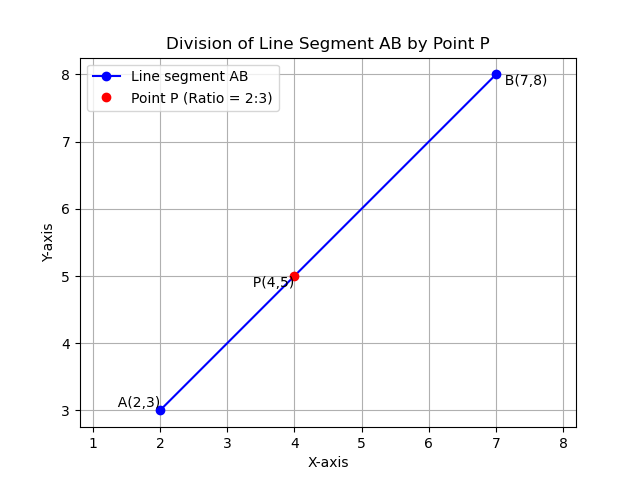
\includegraphics[width=1\linewidth]{fig.png}
 \caption{plot of A,B and P}
 \label{fig:enter-label}
 \end{figure}
 




\end{document}
